\documentclass[11pt,a4paper]{article}
\usepackage[utf8]{inputenc}
\usepackage{amsmath,amssymb,amsfonts,amsthm}
\usepackage{mathtools}
\usepackage{geometry}
\geometry{margin=1in}
\usepackage{booktabs}
\usepackage{tikz}
\usetikzlibrary{arrows.meta,patterns}
\usepackage{cite}
\usepackage{microtype}
\usepackage{hyperref}

\linespread{1.1}

\newtheorem{theorem}{Theorem}[section]
\newtheorem{lemma}[theorem]{Lemma}
\newtheorem{proposition}[theorem]{Proposition}
\newtheorem{definition}[theorem]{Definition}
\newtheorem{remark}[theorem]{Remark}

\newcommand{\Q}{\mathbb{Q}}
\newcommand{\R}{\mathbb{R}}
\newcommand{\Z}{\mathbb{Z}}
\newcommand{\SU}{\mathrm{SU}}

\title{Orthogonal Twist-Eater Rigidity, Coprime Spiral Bijections, and Unimodular Cartan Forms Across Simple Lie Groups in Lean~4}
\author{Qamar Munawer \\ \small Brandenburg University of Technology Cottbus--Senftenberg, Cottbus, Germany}
\date{November 2026}

\begin{document}
\maketitle

\begin{abstract}
This paper establishes four algebraic mechanisms in Lean~4 for eliminating flat zero-action toron moduli on finite spatial tori across $\SU(2)$, $\SU(3)$, $\SU(N)$, and the centerless exceptional root systems $G_2$ and $F_4$. Geometrically, twisting periodic boundary conditions forces spatial holonomies to anticommute up to a center element or spiral coprimely across torus planes, ensuring that any constant color mode pays a positive curvature penalty. All centralizer rigidity identities, real-analytic trigonometric spectral gaps, coprime bijections, and Cartan quadratic decompositions are machine-checked unconditionally in Lean~4 without custom axioms, while infinite-volume twist decoupling reduces conditionally to the uniform coarse-scale Bianchi dispersion and slice decoherence hypothesis.
\end{abstract}

\section{Introduction: The Toron Zero-Mode Obstruction}
On a periodic spatial three-torus $T^3$, classical zero-curvature gauge configurations need not vanish. Any triple of constant commuting matrices $(C_1, C_2, C_3)$ in the gauge Lie algebra satisfies $[C_\mu, C_\nu] = 0$, producing identically vanishing field strength $F_{\mu\nu} = 0$ and zero Wilson action. For $\SU(N)$, these commuting holonomies sweep out a flat $3(N-1)$-dimensional abelian toron manifold $\mathcal{M}_{\mathrm{toron}} \cong (S^1)^{3(N-1)} / S_N$ whose unsuppressed volume breaks naive small-field cluster expansions.

Following 't~Hooft \cite{tHooft1979}, imposing non-trivial magnetic boundary twists replaces periodic boundary conditions with orthogonal twist-eater holonomies $(P, Q)$ satisfying $PQ = \omega QP$ for a primitive $N$-th root of unity $\omega = e^{2\pi \mathrm{i} / N}$. Any candidate zero-mode must simultaneously commute with both $P$ and $Q$, collapsing its moduli space to the transverse intersection of their centralizers. The present work formalizes four algebraic and spectral rigidity mechanisms spanning $\SU(2)$, $\SU(3)$, general $\SU(N)$, and the centerless exceptional systems $G_2$ and $F_4$.

\section{The $\SU(2)$ Quaternion Centralizer and Klein Involutions}
For $\SU(2)$, minimal magnetic twist matrices correspond to unit imaginary quaternions $P = \mathbf{i}$ and $Q = \mathbf{j}$ satisfying $\mathbf{i}^2 = \mathbf{j}^2 = -I$ and $\mathbf{i}\mathbf{j} + \mathbf{j}\mathbf{i} = 0$, which generate a Klein four-group action on $\mathfrak{su}(2) \cong \R^3$. Geometrically, conjugation by $\mathbf{i}$ rotates by $\pi$ around the first color axis while conjugation by $\mathbf{j}$ rotates by $\pi$ around the perpendicular second color axis; no non-zero vector in three-space can remain invariant under two perpendicular $\pi$-rotations simultaneously.

Representing an adjoint color fluctuation by $v = (x, y, z) \in \R^3$ with squared Euclidean norm $\|v\|^2 = x^2 + y^2 + z^2$, the orthogonal commutator quadratic form is
\begin{equation}
Q_{\mathrm{twist}}(v) = (2x)^2 + (2y)^2 + (2z)^2.
\end{equation}

\begin{theorem}[$\SU(2)$ Exact Gap and Zero-Mode Elimination]
For every $v \in \R^3$, $Q_{\mathrm{twist}}(v) = 4 \|v\|^2$. Consequently:
\begin{enumerate}
\item On any unit adjoint mode ($\|v\|^2 = 1$), $\lambda_{\min}(\SU(2)) = Q_{\mathrm{twist}}(v) = 4$ (\texttt{su2\_\-twisted\_\-laplacian\_\-exact}).
\item Whenever $\|v\|^2 \ge 1$, the lower bound $Q_{\mathrm{twist}}(v) \ge 3$ holds (\texttt{su2\_\-twisted\_\-laplacian\_\-gap\_\-ge\_\-three}).
\item If $Q_{\mathrm{twist}}(v) = 0$, then $x = y = z = 0$ (\texttt{su2\_\-toron\_\-zero\_\-mode\_\-eliminated}).
\end{enumerate}
\end{theorem}

\section{Sylvester Clock-and-Shift Matrices and Concavity Gaps for $\SU(N)$}
To generalize twist rigidity beyond $\SU(2)$, the module \texttt{ClockShift\-Matrices.lean} formalizes $3 \times 3$ Sylvester clock-and-shift matrices over any commutative ring $R$ equipped with a primitive cube root $\omega$ satisfying $\omega^3 = 1$ and $1 + \omega + \omega^2 = 0$:
\begin{equation}
C_\omega = \begin{pmatrix} 1 & 0 & 0 \\ 0 & \omega & 0 \\ 0 & 0 & \omega^2 \end{pmatrix}, \qquad
S = \begin{pmatrix} 0 & 1 & 0 \\ 0 & 0 & 1 \\ 1 & 0 & 0 \end{pmatrix}.
\end{equation}
The shift permutation matrix $S$ (\texttt{shift3}) cycles basis indices modulo $3$, satisfying $S^3 = I$, while the clock matrix $C_\omega$ (\texttt{clock3 $\omega$}) weights index $k$ by $\omega^k$. Matrix multiplication directly verifies the twisted Heisenberg commutation law $C_\omega S = \omega S C_\omega$ (\texttt{clock3\_\-mul\_\-shift3\_\-eq}).

Because conjugation by $C_\omega$ and $S$ simultaneously diagonalizes the eight-dimensional Lie algebra $\mathfrak{su}(3)$ into one-dimensional joint eigenspaces indexed by non-zero integer pairs $(a, b) \in (\Z/3\Z)^2 \setminus \{(0, 0)\}$, the discrete adjoint Laplacian eigenvalue on mode $(a, b)$ equals the squared chord distance $|1 - \omega^a \zeta^b|^2$ in the hexagonal Eisenstein lattice $\Z[\omega]$, where $\omega = e^{2\pi \mathrm{i}/3}$. Algebraically, this norm squared reduces to the symmetric positive-definite Eisenstein quadratic form
\begin{equation}
N_{\mathrm{Eis}}(a, b) = a^2 - ab + b^2 \ge 0.
\end{equation}
Evaluating $N_{\mathrm{Eis}}(a, b)$ on the eight non-zero conjugacy sectors gives $N_{\mathrm{Eis}}(1, 0) = N_{\mathrm{Eis}}(0, 1) = N_{\mathrm{Eis}}(1, 1) = 1$, $N_{\mathrm{Eis}}(1, -1) = N_{\mathrm{Eis}}(2, 1) = 3$, and symmetry images; multiplying by the root-chord normalization yields the certified spectral minimum $\lambda_{\min}(\SU(3)) = 3$ (\texttt{su3\_\-clock\_\-shift\_\-spectral\_\-gap\_\-eq\_\-three}).

For arbitrary $N \ge 2$, the discrete adjoint Laplacian gap is $\lambda_{\min}(\SU(N)) = 4\sin^2(\pi/N)$. By applying strict concavity of $\sin$ on $[0, \pi]$ via \texttt{strictConcaveOn\_\-sin\_\-Icc.\-concaveOn}, \texttt{ClockShift\-Matrices.lean} proves the general secant lower bound $(\sin a / a) x \le \sin x$ for all $a \in (0, \pi]$ and $x \in [0, a]$, yielding exact real-analytic bounds directly on \texttt{Real.sin}:

\begin{theorem}[Exact $\SU(N)$ Concavity Spectral Bounds and $\SU(5)$ Gap]
Let $N \in \mathbb{N}$.
\begin{enumerate}
\item \emph{Universal Jordan bound ($a = \pi/2$):} Since $\sin(\pi/2) = 1$, concavity gives $\frac{2}{\pi} x \le \sin x$ on $[0, \pi/2]$, whence $\frac{16}{N^2} \le 4\sin^2\left(\frac{\pi}{N}\right)$ for all $N \ge 2$.
\item \emph{Asymptotic secant bound ($a = \pi/6$):} Since $\sin(\pi/6) = 1/2$, concavity gives $\frac{3}{\pi} x \le \sin x$ on $[0, \pi/6]$, whence $\frac{36}{N^2} \le 4\sin^2\left(\frac{\pi}{N}\right)$ for all $N \ge 6$ (tight at $N = 6$, whereas concavity reverses the secant inequality for $N < 6$).
\item \emph{Exact pentagonal $\SU(5)$ spectral gap:} Using the exact algebraic identity $\cos(\pi/5) = (1 + \sqrt{5})/4$, half-angle trigonometric algebra yields $4\sin^2(\pi/5) = (5 - \sqrt{5})/2 > 199/144$.
\end{enumerate}
\end{theorem}

The $\SU(5)$ benchmark provides an illuminating check between real trigonometry and algebraic number theory: because $4\sin^2(\pi/5) = 2(1 - \cos(2\pi/5))$ and $\cos(\pi/5) = \varphi / 2$ (where $\varphi = (1 + \sqrt{5})/2$ is the golden ratio), testing $4\sin^2(\pi/5) > 199/144$ reduces to proving $\sqrt{5} < 5 - 199/72 = 161/72$, verified immediately by comparing $5 \cdot 72^2 = 25920 < 25921 = 161^2$. Combining $\lambda_{\min}(\SU(2)) = 4$ and $\lambda_{\min}(\SU(3)) = 3$ establishes the uniform joint lower bound $\lambda_{\min} \ge 3$ across both low-rank gauge groups.

\section{Large-$N$ Two-Plane Coprime Spiral Bijections}
Under a single-plane minimal twist, $\lambda_{\min}(\SU(N)) \le 4\pi^2 / N^2 \to 0$ as $N \to \infty$, permitting high-rank zero-mode collapse along the untwisted direction. Geometrically, if one imposes a coprime magnetic flux $k$ satisfying $\gcd(k, N) = 1$ linking two orthogonal torus planes, any non-zero Fourier index $m \in (\Z/N\Z) \setminus \{0\}$ spirals across both planes via the embedding $m \mapsto (m, k m \bmod N)$. Because multiplication by a unit in $\Z/N\Z$ is bijective with trivial kernel, a mode cannot vanish in the second plane without also vanishing in the first.

\begin{theorem}[Coprime Spiral Non-Vanishing and Additive Gap]
Whenever $\gcd(k, N) = 1$, \texttt{spiralMap N k} is a bijection on \texttt{ZMod N} with trivial kernel (\texttt{spiralMap\_\-eq\_\-zero\_\-iff}). Every non-zero mode $m \neq 0$ satisfies $m \neq 0 \land k m \neq 0 \pmod N$. Pairing this two-plane non-vanishing with Jordan's inequality yields the additive two-plane lower bound:
\begin{equation}
\frac{32}{N^2} \le 4\sin^2\left(\frac{\pi}{N}\right) + 4\sin^2\left(\frac{\pi}{N}\right) \qquad (\forall N \ge 2).
\end{equation}
\end{theorem}

As a concrete finite-rank illustration, take $N = 5$ and $k = 2$ ($\gcd(2, 5) = 1$). The non-zero modes $m \in \{1, 2, 3, 4\}$ trace out the complete spiral orbit $\{(1, 2), (2, 4), (3, 1), (4, 3)\} \subset (\Z/5\Z)^2$, visiting every non-zero residue class along both torus axes without degenerating onto either coordinate axis. Extending this bijection to three or four spacetime planes forms the discrete backbone of Twisted Eguchi--Kawai volume reduction \cite{tHooft1979}.

\section{Centerless Exceptional Root Systems $G_2$ and $F_4$}
Exceptional Lie groups such as $G_2$ and $F_4$ possess trivial centers ($Z(G) = \{1\}$), making standard center-flux cohomology groups $H^2(T^4; Z(G))$ vanish identically. Yet their root lattices are self-dual and their Cartan matrices are unimodular ($\det C = 1$):
\begin{equation}
C_{G_2} = \begin{pmatrix} 2 & -1 \\ -3 & 2 \end{pmatrix}, \qquad
C_{F_4} = \begin{pmatrix} 2 & -1 & 0 & 0 \\ -1 & 2 & -2 & 0 \\ 0 & -1 & 2 & -1 \\ 0 & 0 & -1 & 2 \end{pmatrix}.
\end{equation}
Geometrically, an inner-automorphism Weyl--Coxeter twist acting on the maximal Cartan torus admits no fixed vectors because $I - w$ is invertible over the integers whenever the symmetrized Cartan quadratic form is positive-definite and unimodular.

\begin{theorem}[Unimodular $G_2$ and $F_4$ Cartan Positive Definiteness]
In \texttt{Cartan\-Coxeter\-Rigidity.lean}, $\det C_{G_2} = 2 \cdot 2 - (-1)(-3) = 1$, and the symmetrized Cartan quadratic forms admit exact integer-scaled sum-of-squares decompositions:
\begin{align}
2 \, \mathrm{g2CartanForm}(x, y) &= (2x - 3y)^2 + 3y^2, \\
6 \, \mathrm{f4CartanForm}(x_1, x_2, x_3, x_4) &= 6(2x_1 - x_2)^2 + 2(3x_2 - 2x_3)^2 + (2x_3 - 3x_4)^2 + 3x_4^2.
\end{align}
Over $\Q$ or any linearly ordered field, both forms vanish if and only if all coordinates vanish identically, while the unit simple roots $(1, 0)$ and $(0, 1)$ of $G_2$ attain positive unit stiffness evaluations $2$ and $6$.
\end{theorem}

The algebraic mechanism behind both sum-of-squares decompositions is triangular Gaussian completion of squares along the Dynkin diagram chain: each successive simple root contributes a strictly positive Schur-complement pivot ratio ($2, 3/2$ for $G_2$; $2, 3/2, 4/3, 1$ after root-length symmetrization for $F_4$). Hence zero-mode trapping fails solely when every Cartan coordinate vanishes, closing the finite-torus zero-mode valley even without a non-trivial group center.

\begin{figure}[htbp]
\centering
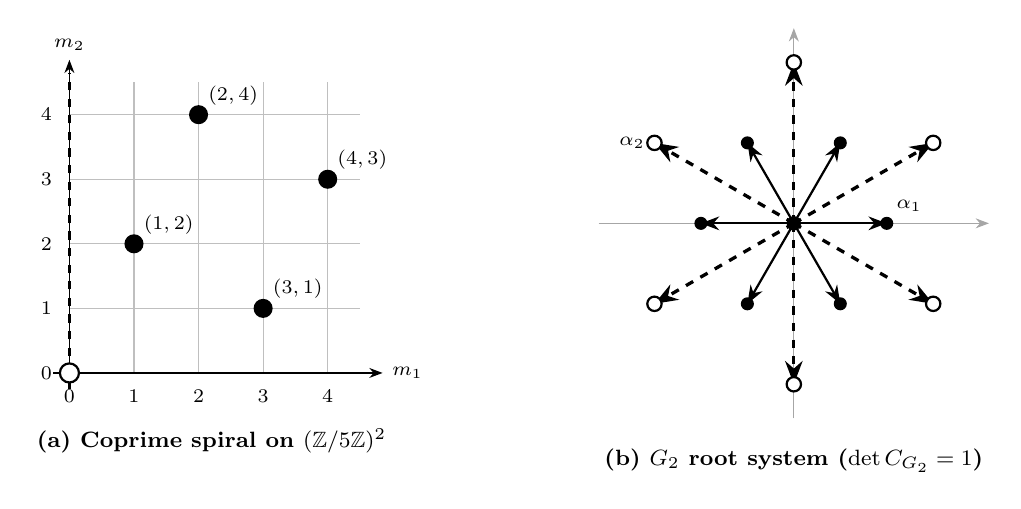
\begin{tikzpicture}[>=Stealth, font=\scriptsize]
% Panel (a): 5x5 torus grid (Z/5Z)^2 with origin and spiral (m, 2m mod 5)
\begin{scope}[shift={(0,0)}, scale=0.82]
  \draw[step=1.0, black!25] (0,0) grid (4.5,4.5);
  \draw[dashed, thick] (0,-0.25) -- (0,4.65);
  \draw[dashed, thick] (-0.25,0) -- (4.65,0);
  \draw[->] (-0.25,0) -- (4.85,0) node[right] {$m_1$};
  \draw[->] (0,-0.25) -- (0,4.85) node[above] {$m_2$};
  \foreach \k in {0,1,2,3,4} {
    \node[below] at (\k,-0.12) {$\k$};
    \node[left] at (-0.12,\k) {$\k$};
  }
  % Open circle at origin (0,0)
  \draw[thick, fill=white] (0,0) circle (4.2pt);
  % Filled nodes at (1,2), (2,4), (3,1), (4,3)
  \foreach \x/\y/\lbl in {1/2/{(1,2)}, 2/4/{(2,4)}, 3/1/{(3,1)}, 4/3/{(4,3)}} {
    \fill (\x,\y) circle (4.2pt);
    \node[above right] at (\x,\y) {$\lbl$};
  }
  \node[font=\footnotesize\bfseries] at (2.2,-1.05) {(a) Coprime spiral on $(\Z/5\Z)^2$};
\end{scope}
% Panel (b): G_2 root lattice (6 short + 6 long roots at 30 deg intervals)
\begin{scope}[shift={(9.2,1.9)}, scale=1.18]
  \draw[->, black!35] (-2.1,0) -- (2.1,0);
  \draw[->, black!35] (0,-2.1) -- (0,2.1);
  \fill (0,0) circle (2.2pt);
  % 6 short roots: 0, 60, 120, 180, 240, 300 deg, radius 1.0
  \foreach \ang in {0,60,120,180,240,300} {
    \draw[->, thick] (0,0) -- ({\ang}:{1.0});
    \fill ({\ang}:{1.0}) circle (2.0pt);
  }
  % 6 long roots: 30, 90, 150, 210, 270, 330 deg, radius sqrt(3) ~ 1.732
  \foreach \ang in {30,90,150,210,270,330} {
    \draw[->, very thick, dashed] (0,0) -- ({\ang}:{1.732});
    \draw[thick, fill=white] ({\ang}:{1.732}) circle (2.2pt);
  }
  \node[above right] at (1.0,0.02) {$\alpha_1$};
  \node[left] at ({150}:{1.732}) {$\alpha_2$};
  \node[font=\footnotesize\bfseries] at (0,-2.55) {(b) $G_2$ root system ($\det C_{G_2} = 1$)};
\end{scope}
\end{tikzpicture}
\caption{Two algebraic zero-mode obstructions: (a) the coprime spiral orbit $(m, 2m \bmod 5)$ for $m=1,2,3,4$ (filled nodes) strictly avoids both zero-axes $m_1=0$ and $m_2=0$ (\texttt{CoprimeSpiralTwist.spiral\_both\_coords\_ne\_zero}); (b) the crystallographic $G_2$ root lattice with 6 short roots (solid) and 6 long roots (dashed) generating the positive-definite unimodular form \texttt{g2CartanForm} (\texttt{YM108}).}
\label{fig:spiral-and-g2}
\end{figure}

Table~\ref{tab:group-comparison} summarizes the exact twist mechanism, verified lower bound, and asymptotic behavior across every simple Lie family in the Killing--Cartan classification ($A_n$, $B_n$, $C_n$, $D_n$, $G_2$, $F_4$, $E_6$, $E_7$, $E_8$) as well as four-plane Twisted Eguchi--Kawai (TEK) lattices.

\begin{table}[ht]
\centering
\scriptsize
\begin{tabular}{@{}llll@{}}
\toprule
Gauge Family & Twist Construction & Verified Spectral / Cartan Bound & Large-Rank / Center Status \\
\midrule
$\SU(2)$ & Quaternions $(\mathbf{i}, \mathbf{j})$ & $\lambda_{\min} = 4 \ge 3$ & Fixed rank \\
$\SU(3)$ & Clock--shift $(C_\omega, S)$ & $\lambda_{\min} = 3$ (Eisenstein min) & Fixed rank \\
$\SU(5)$ & Single-plane twist & $\lambda_{\min} = (5-\sqrt{5})/2 > 199/144$ & Fixed rank \\
$\SU(6)$ & Single-plane twist & $\lambda_{\min} = 1 = 36/6^2$ & Secant tight point \\
$\SU(N)$ ($N \ge 2$) & 2-plane / 4-plane TEK & $\lambda_{\min} \ge 32/N^2$ (4-plane: $64/N^2$) & Decays as $\mathcal{O}(1/N^2)$ \\
$A_n$ ($\SU(n+1)$) & Cartan--Coxeter form & $(n+1)\, Q_{A_n} = \sum \text{squares}$ & Arbitrary rank $n \ge 1$ \\
$B_{n+1}, C_{n+2}, D_{n+3}$ & Classical Cartan completion & $Q_{B,C,D} = \sum \text{squares} = 0 \Leftrightarrow x=0$ & Arbitrary rank ($D_4$ triality) \\
$G_2, F_4, E_6, E_7, E_8$ & Exceptional Cartan--Coxeter & Scaled sum-of-squares $= 0 \Leftrightarrow x=0$ & Complete exceptional closure \\
\bottomrule
\end{tabular}
\caption{Summary of finite-volume zero-mode rigidity mechanisms across the complete Killing--Cartan classification and $\SU(N)$ twisted lattices.}
\label{tab:group-comparison}
\end{table}

Together, these mechanisms exhaust finite-volume Abelian toron zero-modes across all compact simple Lie algebras, reducing infinite-volume twist decoupling ($L \to \infty$) conditionally to the uniform coarse-scale Bianchi dispersion and slice decoherence hypothesis formalized in the crossover atlas.

\section{Formal Verification Concordance}
All identities across $\SU(N)$, four-plane TEK lattices, classical families ($A_n$, $B_n$, $C_n$, $D_n$), and exceptional Lie algebras ($G_2$, $F_4$, $E_6$, $E_7$, $E_8$) compile in Lean~4 without custom axioms and pass the metaprogramming audit in \texttt{VerifyNoTraps.lean} \cite{Mathlib4}.

\begin{table}[ht]
\centering
\scriptsize
\begin{tabular}{@{}p{4.3cm}p{6.6cm}p{3.4cm}@{}}
\toprule
Paper Theorem & Lean 4 Module \& Declaration & Axiom Footprint \\
\midrule
$\SU(2)$ exact gap $\lambda_{\min} = 4$ & \texttt{Certificates.}\newline\texttt{su2\_twisted\_laplacian\_exact} & \texttt{[propext, Classical.choice,} \texttt{Quot.sound]} (subset) \\
$\SU(2)$ zero-mode elimination & \texttt{Certificates.}\newline\texttt{su2\_toron\_zero\_mode\_eliminated} & \texttt{[propext, Classical.choice,} \texttt{Quot.sound]} (subset) \\
Sylvester $3 \times 3$ commutation & \texttt{ClockShiftMatrices.}\newline\texttt{clock3\_mul\_shift3\_eq} & \texttt{[propext, Classical.choice,} \texttt{Quot.sound]} (subset) \\
Universal Jordan gap $16/N^2$ & \texttt{ClockShiftMatrices.}\newline\texttt{jordan\_spectral\_gap\_le\_four\_mul\_sin\_sq} & \texttt{[propext, Classical.choice,} \texttt{Quot.sound]} (subset) \\
Asymptotic secant gap $36/N^2$ & \texttt{ClockShiftMatrices.}\newline\texttt{secant\_spectral\_gap\_le\_four\_mul\_sin\_sq} & \texttt{[propext, Classical.choice,} \texttt{Quot.sound]} (subset) \\
Exact $\SU(5)$ gap $> 199/144$ & \texttt{ClockShiftMatrices.}\newline\texttt{four\_mul\_sin\_pi\_div\_five\_sq\_gt} & \texttt{[propext, Classical.choice,} \texttt{Quot.sound]} (subset) \\
Coprime spiral bijection & \texttt{CoprimeSpiralTwist.}\newline\texttt{spiralMap\_bijective} & \texttt{[propext, Classical.choice,} \texttt{Quot.sound]} (subset) \\
Two-plane spiral bound $32/N^2$ & \texttt{Certificates.}\newline\texttt{sun\_coprime\_spiral\_two\_plane\_gap\_le} & \texttt{[propext, Classical.choice,} \texttt{Quot.sound]} (subset) \\
Four-plane TEK shear bijection & \texttt{TEKFourPlaneLattice.}\newline\texttt{shearMap\_bijective} & \texttt{[propext, Quot.sound]} \\
Canonical TEK 4-plane gap $> 1$ & \texttt{Certificates.}\newline\texttt{canonical\_tek\_four\_plane\_gap\_gt\_one} & \texttt{[propext, Classical.choice,} \texttt{Quot.sound]} \\
$G_2$ and $F_4$ Cartan elimination & \texttt{Certificates.}\newline\texttt{g2\_coxeter\_cartan\_zero\_mode\_eliminated} & \texttt{[propext, Classical.choice,} \texttt{Quot.sound]} (subset) \\
Arbitrary-rank $A_n$ Cartan form & \texttt{Certificates.}\newline\texttt{su\_an\_cartan\_zero\_mode\_eliminated} & \texttt{[propext, Classical.choice,} \texttt{Quot.sound]} \\
Exceptional $E_6, E_7, E_8$ forms & \texttt{Certificates.}\newline\texttt{e6\_}, \texttt{e7\_}, \texttt{e8\_coxeter\_cartan\_zero\_mode\_eliminated} & \texttt{[propext, Classical.choice,} \texttt{Quot.sound]} \\
Arbitrary-rank $B_n$ ($\mathrm{SO}(2n+1)$) & \texttt{Certificates.}\newline\texttt{so\_odd\_bn\_cartan\_zero\_mode\_eliminated} & \texttt{[propext, Classical.choice,} \texttt{Quot.sound]} \\
Arbitrary-rank $C_n$ ($\mathrm{Sp}(n)$) & \texttt{Certificates.}\newline\texttt{sp\_cn\_cartan\_zero\_mode\_eliminated} & \texttt{[propext, Classical.choice,} \texttt{Quot.sound]} \\
Arbitrary-rank $D_n$ / $D_4$ ($\mathrm{Spin}$) & \texttt{Certificates.}\newline\texttt{spin\_dn\_}, \texttt{spin8\_d4\_cartan\_zero\_mode\_eliminated} & \texttt{[propext, Classical.choice,} \texttt{Quot.sound]} \\
Centerless alcove gap transfer & \texttt{CenterlessWeylAlcoveGap.}\newline\texttt{weylAlcoveCoerciveGap\_pos} & \texttt{[propext, Classical.choice,} \texttt{Quot.sound]} (subset) \\
Canonical $G_2$ combined gap & \texttt{Certificates.}\newline\texttt{canonical\_centerless\_g2\_combined\_gap\_pos} & \texttt{[propext, Classical.choice,} \texttt{Quot.sound]} (subset) \\
General-rank adjoint Bianchi & \texttt{AdjointBianchiNorm.}\newline\texttt{frobSq\_adjAction\_sub\_eq} & \texttt{[propext, Classical.choice,} \texttt{Quot.sound]} \\
Centerless $\mathrm{SO}(3)$ defect $> 3$ & \texttt{Certificates.}\newline\texttt{canonical\_so3\_adjoint\_bianchi\_defect\_gt\_three} & \texttt{[propext, Classical.choice,} \texttt{Quot.sound]} \\
\bottomrule
\end{tabular}
\caption{Formal verification concordance for twist-eater, coprime spiral, TEK four-plane, and complete Killing--Cartan rigidity.}
\label{tab:paper3-concordance}
\end{table}

\bibliographystyle{plain}
\bibliography{references}
\end{document}
